\documentclass[]{article}
\usepackage{geometry}   % my added package "geometry"
\geometry{letterpaper,tmargin=1in,bmargin=1in,lmargin=2.2cm,rmargin=2.2cm}
\usepackage[colorlinks,bookmarksopen,bookmarksnumbered,
citecolor=green,urlcolor=red]{hyperref}
\hypersetup{pdfauthor={Name}}
%%%%%%%%%%%%%%%%%%%%%%%%%%%%%%%%%%%%%%%%%%%%%%%%%%%%%%%%%%%%%%%%%%%%%%%%%
%\usepackage{graphicx}
\usepackage{graphics}
\usepackage{epsfig}
\usepackage{epstopdf}
\usepackage{amsfonts}
\usepackage{amssymb}
\usepackage{booktabs}
\usepackage{color,soul}
%%%%%%%%%%%%%%%%%%%%%%%%%%%%%%%%%%%%%%%%%%%%%%%%%%%%%%%%%%%%%%%%%
\usepackage{amsmath}
\usepackage{cleveref}
\usepackage{authblk}
%\usepackage[fleqn]{amsmath}
\usepackage{lineno}
\usepackage{tikz}
\usepackage{standalone}
\usetikzlibrary{calc,patterns,arrows.meta,shapes.arrows,intersections,positioning}
\usetikzlibrary{decorations.pathmorphing,backgrounds,fit,petri}
\usepackage[percent]{overpic}
%%%%%%%%%%%%%%%%%%%%%%%%%%%%%%%%%%%%%%%%%%%%%%%%%%%%%%%%%%%%%%%%%
\usepackage{xcolor}
\usepackage{listings}
\lstset { %
	language=C++,
	backgroundcolor=\color{blue!5}, % set backgroundcolor
	basicstyle=\footnotesize\color{black},% basic font settingbasicstyle=\ttfamily\color{black}
	keywordstyle=\color{red},
	commentstyle=\color{violet},
	stringstyle=\color{blue},
	xleftmargin=2em,
	frame=single,
	framexleftmargin=2em,
	numbers=left,
	numberstyle=\tiny,
	numbersep=8pt,
}
%%%%%%%%%%%%%%%%%%%%%%%%%%%%%%%%%%%%%%%%%%%%%%%%%%%%%%%%%%%%%%%%%
\renewcommand\thesubsection{\thesection\Alph{subsection}}
%%%%%%%%%%%%%%%%%%%%%%%%%%%%%%%%%%%%%%%%%%%%%%%%%%%%%%%%%%%%%%%%%
\renewcommand\lstlistingname{Header}
\renewcommand\lstlistlistingname{Header}
%%%%%%%%%%%%%%%%%%%%%%%%%%%%%%%%%%%%%%%%%%%%%%%%%%%%%%%%%%%%%%%%%%%%
%opening
\begin{document}
\title{HiperLife Tutorial: Nonlinear Poisson}
\author{Arash Imani}
\affil{LaCàN}
\maketitle

\linenumbers

\section{Problem Definition} \label{sec: pd} 
The nonlinear Poisson equations are significantly more challenging to solve than its linear counterpart because the relationship between the potential and source term is complex. Understanding and solving the nonlinear Poisson equation is essential for designing and optimizing devices, interpreting material behaviors, and simulating natural processes in many areas of physics and engineering.
\begin{figure}[htbp]
	\centering
	
\documentclass[preprint,12pt,a4]{standalone}
\usepackage{geometry}   % my added package "geometry"
\geometry{letterpaper,tmargin=1in,bmargin=1in,lmargin=2.5cm,rmargin=2.5cm}
\usepackage{tikz}
\usetikzlibrary{calc,patterns,arrows.meta,shapes.arrows,intersections,positioning}
\usetikzlibrary{decorations.pathmorphing,backgrounds,fit,petri}
\usepackage{standalone}
\begin{document}
	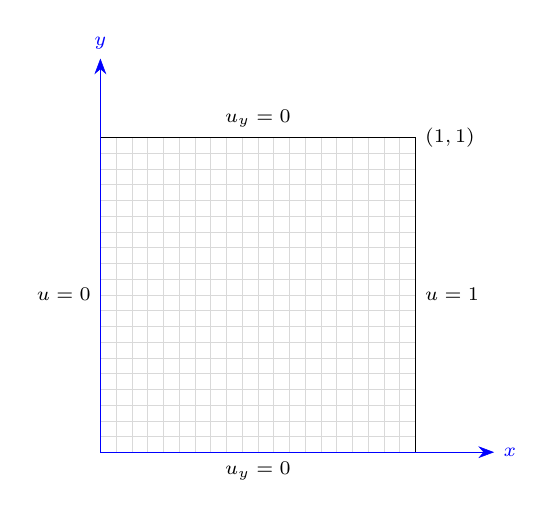
\begin{tikzpicture} [{place/.style={rectangle,draw=blue!50,fill=blue!20,ultra thin,inner sep=0.8mm}},{place2/.style={circle,draw=black!50,ultra thin,inner sep=0.8mm}},{linest/.style={color=gray,ultra thin}}]
	%%coordinates of corners of Beam
	\coordinate (A) at (0,0);
	\coordinate (B) at (2,0);
	\coordinate (C) at (4,0);
	\coordinate (D) at (4,2);
	\coordinate (E) at (4,4);
	\coordinate (F) at (2.0,4);
	\coordinate (G) at (0.0,4);
	\coordinate (H) at (0.0,2);
	%%mesh
	\draw [line width=0.1pt,gray!30,step=2mm](A) grid (E);
	%%Beam	
	\draw [color=black](A)-- (B)node [below,color = black,font=\scriptsize] {$u_y=0$}--(C)--(D)node [right,color = black,font=\scriptsize] {$u=1$}--(E)node [right,color = black,font=\scriptsize] {$(1,1)$}--(F)node [above,color = black,font=\scriptsize] {$u_y=0$}--(G)--(H)node [left,color = black,font=\scriptsize] {$u=0$}--(A);
	
	%%axes
	\draw [-{Stealth[length=2mm]},help lines,blue] (A) -> (5,0) node [right,color = blue,font=\scriptsize] {$x$};
		\draw [-{Stealth[length=2mm]}, help lines,blue] (A) -- (0,5) node [above,color = blue,font=\scriptsize] {$y$};

	\end{tikzpicture}
\end{document}
	\caption{Geometry, BC and computational domain used for the analysis of nonlinear Poisson.}
	\label{fig_SB}
\end{figure}

The exact solution for this particular problem is given by
\begin{equation}\label{eq1}
	\begin{aligned}
		u(x,y) = (3x +1)^{1/2}-1\thinspace .
	\end{aligned}
\end{equation}
Here we want to use finite element method to solve it. Because in general unlike linear equations, solutions cannot be directly superimposed, and standard analytical methods like separation of variables are usually not applicable for nonlinear type. Instead, specialized techniques such as variational approaches, and numerical methods are employed to tackle these problems.
\section{Governing Equations} \label{sec: ge}
In this section we present the governing equations, consider this nonlinear PDE:\cite{BarattaEtal2023}
\begin{equation}\label{eq2}
	\begin{aligned}
		- \nabla \cdot [(1+u)\nabla u] = f \quad \text{in} \ \Omega
	\end{aligned}
\end{equation}
As it is demonstrated in Figure \ref{fig_SB}, The domain $\Omega$ is a square of dimensions $[0,1] \times [0,1]$ along the $x$ and $y$ coordinates, where $f = 0$ and the boundary conditions to be
\begin{equation}\label{eq3}
	\begin{aligned}
		u(0,y) &= 0, \ u(1,y) = 1\quad \text{on} \ \Gamma_D \\
		u_y(x,0) &=u_y(x,1) =0 \quad \text{on} \ \Gamma_N \\
	\end{aligned}
\end{equation}
\section{Weak Form} \label{sec: wf}
The starting point for the development of the finite element models of Eq. (\ref{eq1}) is their weak forms.
The variational formulation of our model problem reads: Find $u \in V$ such that
\begin{equation}\label{eq4}
	\begin{aligned}
		\mathcal{F}(u;v) = 0 \quad \forall v \in \hat{V}
	\end{aligned}
\end{equation}
where
\begin{equation}\label{eq5}
	\begin{aligned}
		\mathcal{F}(u; v) =-\int_\Omega v \nabla \cdot[(1+u) \nabla u] - v f \mathrm{d}\Omega\thinspace .
	\end{aligned}
\end{equation}
and
\begin{equation}\label{eq6}
	\begin{aligned}
		\hat{V} &= \{v \in H^1(\Omega) : v = 0 \text{ on } x=0\mbox{ and }x=1\}, \\
		V &= \{v \in H^1(\Omega) : v = 0 \text{ on } x=0\text{ and } v = 1\text{ on }x=1\}\thinspace.
	\end{aligned}
\end{equation}
where $v$ is a test function, which will be equated, in the our FE model to the interpolation function used for $u$.The discrete problem arises as usual by restricting $V$ and $\hat{V}$ to a pair of discrete spaces. Since $\mathcal{F}$ is a nonlinear function of $u$, the variational statement gives rise to a system of nonlinear algebraic equations. using integrating by part this expression over $\Omega$, we have
\begin{equation}\label{eq7}
	\begin{aligned}
		\mathcal{F}(u; v) = -\int_{\Omega} \nabla \cdot [v (1+u) \nabla u] + \int_{\Omega}  (1+u)\nabla v\nabla u - \int_{\Omega} v f \mathrm{d}\Omega\thinspace .
	\end{aligned}
\end{equation}
Using Gauss’s theorem we get
\begin{equation}\label{eq8}
	\begin{aligned}
		\mathcal{F}(u; v) =  -\int_{\Gamma} [v (1+u^2) \nabla u] \cdot n \ \mathrm{d} \Gamma + \int_{\Omega} (1+u)\nabla u \nabla v \mathrm{d} \Omega - \int_{\Omega} v f \mathrm{d} \Omega\thinspace .
	\end{aligned}
\end{equation}
Applying boundary conditions ($\Gamma = \Gamma_N \cup \Gamma_D$):
\begin{equation}\label{eq9}
	\begin{aligned}
		v= 0 \quad &\text{ on } \Gamma_D\thinspace, \\
		\nabla u \cdot n = 0 \quad &\text{ on } \Gamma_N \thinspace.
	\end{aligned}
\end{equation}

and by assuming $f=0$ we get the final form for $\mathcal{F}$
\begin{equation}\label{eq10}
	\begin{aligned}
		\mathcal{F}(u; v) = \int_\Omega (1+u)\nabla u\cdot \nabla v \, \mathrm{d}\Omega,
	\end{aligned}
\end{equation}
After having discretized our nonlinear PDE problem, we now need to linearize it, we may use Newton’s method to solve the system of nonlinear algebraic equations. Newton’s method for the system $\mathcal{F}_i(U_1,\ldots,U_j)$ can be formulated by the first terms of a Taylor series approximation for the value of the variational as
\begin{equation}\label{eq11}
	\begin{aligned}
		\sum_{j=1}^N {\partial \over\partial U_j} \mathcal{F}_i(U_1^k,\ldots,U_N^k)\delta U_j &= -\mathcal{F}_i(U_1^k,\ldots,U_N^k),\quad i=1, \ldots ,N,\\ U_j^{k+1} &= U_j^k + \delta U_j,\quad j=1, \ldots ,N,
	\end{aligned}
\end{equation}
where $k$ is an iteration index. An initial guess $u^0$ must be provided to start the algorithm. We need to compute the $\partial \mathcal{F}_i/\partial U_j$ and the right-hand side vector $-\mathcal{F}_i$. Our present problem has $\mathcal{F}_i$ given by above. so, Hessian is given by
\begin{equation}\label{eq12}
	\begin{aligned}
		\mathcal{J}(u;\phi_j,\phi_i) = {\partial F_i\over\partial U_j} = \int_\Omega \left\lbrack \frac{\partial u}{\partial U_j} \nabla u^k \cdot \nabla v + (1+u^k) \nabla [\frac{\partial u}{\partial U_j}] \cdot \nabla v \right\rbrack \, \mathrm{d}\Omega\thinspace .
	\end{aligned}
\end{equation}
\section{Finite Element Model} \label{sec: fem}
For Ritz-Galerkin FE model, the choice of the test functions is restricted to the spaces of approximation functions used for the solution field. Suppose that the variable $u$ approximated by expansions of the form
\begin{equation}\label{eq13}
	\begin{aligned}
		u(\mathbf{x}, t)= \sum_{j=1}^{M} \phi_j(\mathrm{x}) u_j(t) = \boldsymbol{\Phi}^T\mathbf{u} \thinspace.
	\end{aligned}
\end{equation}

By considering Eq. (\ref{eq13}), the Hessian ($\mathcal{J}=\partial \mathcal{F}_i/\partial U_j$) can be introduced in this way
\begin{equation}\label{eq14}
	\begin{aligned}
		\mathcal{J}(u;\phi_j,\phi_i) = {\partial F_i\over\partial U_j} = \int_\Omega \left\lbrack \phi_j \nabla u^k \cdot \nabla \phi_i + (1+u^k) \nabla \phi_j \cdot \nabla \phi_i \right\rbrack \, \mathrm{d}\Omega\thinspace .
	\end{aligned}
\end{equation}
The above equations can be written symbolically in matrix form as
\begin{equation}\label{eq15}
	\begin{aligned}
		\mathbf{K}\mathbf{\theta} = \mathbf{F}\thinspace.
	\end{aligned}
\end{equation}
In the Hiperlife legacy codes the coefficient matrices $\mathbf{K}$ and $\mathbf{F}$  shown in Eq. (\ref{15}) are defined as Hessain and Jacobian, respectively. In this problem they are given by
\begin{equation}\label{eq16}
	\begin{aligned}
		\mathbf{K}_{ij} &= \int_{\Omega^e} \left\lbrack \phi_j \nabla u^k \cdot \nabla \phi_i + (1+u^k) \nabla \phi_j \cdot \nabla \phi_i \right\rbrack\mathrm{d}A\thinspace,\\
		\mathbf{F}_i &=-\int_{\Omega^e} [(1+u^k)\nabla u^k\cdot \nabla \phi_i]\mathrm{d}A \thinspace.
	\end{aligned}
\end{equation}

The elemental representation of the vector and matrix required for implementation in the Hiperlife would be like\footnote{Note that HiperLife by default applies the $-$ in $Bk(i)$ to Nonlinear problems, so it is not required to add it to your code!}
\begin{equation}\label{eq17}
	\begin{aligned}[b]
		Bk(i) &= -\mathcal{F}_i = \mathcolor{red}{-}jac \times[(1+u^k)\nabla u^k\cdot \nabla \phi_i], \\
		Ak(i,j) &=  \mathcal{J}_{ij} = jac \times [\phi_j \nabla u^k \cdot \nabla \phi_i + (1+u^k) \nabla \phi_j \cdot \nabla \phi_i]\thinspace .
	\end{aligned}
\end{equation}
Note that $dA=dx_{1} \times dx_{2}=jac \ d\xi d\eta$, which $jac=\mathrm{det}(Jacobian)$.
\section{Choice of Elements} \label{sec: coe}
Thus, for this simple problem every Lagrange and serendipity family of interpolation functions are admissible for the interpolation of the temperature field, our choice is would be linear quadrilateral element.Linear  Quadrilateral Elements is the simplest quadrilateral element consists of four nodes. The associated interpolation functions for geometry and field variables are bilinear.
\begin{equation}\label{eq18}
	\begin{aligned}[b]
		\boldsymbol{\Phi}_{I}(\xi, \eta) = \frac{1}{4}(1+\xi_I\xi)(1+\eta_I\eta) \quad (I \ \text{from} \ 1 \ \text{to} \ 4)
	\end{aligned}
\end{equation}

where $\xi_{I}$ and $\eta_{I}$ are the corner coordinates at element $T$ in domain of $\Omega_{T} \in (-1,1)^2$. As it shown in Figure \ref{fig_el} we are using $2 \times 2$ Gauss–Legendre quadrature integration.
\begin{figure}[htbp]
	\centering
	\documentclass[preprint,12pt,a4]{standalone}
\usepackage{geometry}   % my added package "geometry"
\geometry{letterpaper,tmargin=1in,bmargin=1in,lmargin=2.5cm,rmargin=2.5cm}
\usepackage{tikz}
\usetikzlibrary{calc,patterns,arrows.meta,shapes.arrows,intersections,positioning}
\usetikzlibrary{decorations.pathmorphing,backgrounds,fit,petri}
\usepackage{standalone}
%
\begin{document}
	\begin{tikzpicture} [{place/.style={rectangle,draw=blue!50,fill=blue!20,ultra thin,inner sep=0.8mm}},{place2/.style={circle,draw=black!50,ultra thin,inner sep=0.8mm}},{linest/.style={color=gray,ultra thin}}]
		%axes
		\draw [{Stealth[length=2mm]}-{Stealth[length=2mm]}, help lines,blue] (5.0,0)node[above,font=\scriptsize]{$\xi$} -- (0.0,0.0) -- (0.0,5.0)node[right,font=\scriptsize] {$\eta$};
		%%corner nodes
		\node at (0.0,0.0) [place,fill=violet!60] (1) {};
		\node at (4.0,0.0) [place,fill=violet!60] (2) {};
		\node at (4.0,4.0) [place,fill=violet!60] (3) {};
		\node at (0.0,4.0) [place,fill=violet!60] (4) {};
		%% integration points
	    \node at (1.0,1.0) [place2,fill=gray!60] (5) {};
		\node at (3.0,1.0) [place2,fill=gray!60] (6) {};
		\node at (1.0,3.0) [place2,fill=gray!60] (7) {};
		\node at (3.0,3.0) [place2,fill=gray!60] (8) {};
		%%element border
		\draw [-,black] (1) -- (2) -- (3) -- (4) --(1);
		%%middle nodes
		\node at (5.6,2.5) [right,font=\scriptsize]{$\mathrm{Element \ nodes}$};
		\node at (5.5,2.5) [place,fill=violet!60] (4) {};
		\node at (5.6,2.2) [right,font=\scriptsize]{$\mathrm{integration \ points}$};
		\node at (5.5,2.2) [place2,fill=gray!60] (4) {};
		
	\end{tikzpicture}
\end{document}
	\caption{Linear quadrilateral element used for finite element model.}
	\label{fig_el}
\end{figure}
We also chose a uniform mesh of size $10 \times 10$ to model the domain of our problem.
\section{Implementation} \label{sec: imp}
In this section, we present the implementation of our solution in the Hiperlife. The program is divided into three separate files, main part which we create our problem by the Hiperlife headers, auxiliary header where we introduce parameters and declare defined functions, and at last auxiliary file, where we define some functions which provide required matrices like the Jacobian and the Hessian.
\subsubsection{PoissonNonL.cpp} \label{sec: m.cpp}
\nolinenumbers
\begin{lstlisting}
/*
* nonlinear Poisson equation (using nonlinear solver)
*/
	
// C++ headers
#include <iostream>
#include <fstream>
#include <time.h>
	
// hiperlife headers
#include "hl_Core.h"
#include "hl_Parser.h"
#include "hl_TypeDefs.h"  
#include "hl_DOFsHandler.h"
#include "hl_HiPerProblem.h"
#include "hl_SurfLagrParam.h"
#include "hl_FillStructure.h"
#include "hl_ParamStructure.h"
#include "hl_DistributedMesh.h" 
#include "hl_StructMeshGenerator.h" 
#include "hl_GlobalBasisFunctions.h"
#include "hl_NonlinearSolver_NewtonRaphson.h"
#include "hl_LinearSolver_Iterative_AztecOO.h"
#include <hl_ConsistencyCheck.h>
	
	
// problem header
#include "AuxPoissonNonL.h"
	
int main(int argc, char** argv)
{
	using namespace std;
	using namespace hiperlife;
		
	// **************************************************************//
	/// *****                 INITIALIZATION                    **** ///
	// **************************************************************//
		
	// Initialize the MPI execution environment
	hiperlife::Init(argc, argv);
		
	// Define parameters of the model
	SmartPtr<ParamStructure> paramStr = CreateParamStructure<PoissonParams>();
	double f  = paramStr->getRealParameter(PoissonParams::f);
		
	// **************************************************************//
	// *****                  MESH CREATION                     *****//
	// **************************************************************//
		
	// Create structured mesh
	SmartPtr<StructMeshGenerator> mesh = Create<StructMeshGenerator>();
	mesh->setNDim(3);
	mesh->setElemType(ElemType::Square);
	mesh->setBasisFuncType(BasisFuncType::Lagrangian);
	mesh->setBasisFuncOrder(1);
	mesh->genSquare(10,1.0);
		
	// Distributed mesh
	SmartPtr<DistributedMesh> disMesh = Create<DistributedMesh>();
	disMesh->setMesh(mesh);
	disMesh->setBalanceMesh(true);
	disMesh->setElementLocatorEngine(ElementLocatorEngine::BoundingVolumeHierarchy);
		disMesh->Update();
		
	// checking mesh
	disMesh->printFileLegacyVtk("mesh");
		
	// **************************************************************//
	// *****               DOFsHANDLER CREATION                 *****//
	// **************************************************************//
		
	// Create DOFsHandler
	SmartPtr<DOFsHandler> dofHand = Create<DOFsHandler>(disMesh);
	dofHand->setNameTag("dofHand");
	dofHand->setNumDOFs(1);
	dofHand->setDOFs({"u"});
	dofHand->Update();
		
	// -------------- initial condition first guess ----------------- //
	//----------------------------------------------------------------//
	for (int i = 0; i < disMesh->loc_nPts(); i++)
	{
		// Coordinate
		std::vector<double> x = disMesh->nodeCoords(i, IndexType::Local);
		// Initial condition
		dofHand->nodeDOFs->setValue("u", i, IndexType::Local, x[0]);
		// ---------------------- Boundary condition ---------------- //
		//------------------------------------------------------------//
		if (x[0] < 1e-5)
		{
			dofHand->nodeDOFs->setValue("u", i, IndexType::Local,0.0);
			dofHand->setConstraint("u",i, IndexType::Local,0.0);
		}
		if (x[0] > (1.-1e-5))
		{
			dofHand->nodeDOFs->setValue("u", i, IndexType::Local,1.0);
			dofHand->setConstraint("u",i, IndexType::Local,0.0);
		}
	}
		
	// Update 
	dofHand->UpdateGhosts();
		
	// checking initial and boundary condition
	dofHand->printFileLegacyVtk("PoissonNonL0");
		
	// *************************************************************  //
	/// *****               HIPERPROBLEM CREATION               **** ///
	// *************************************************************  //
		
	// Create hiperproblem
	SmartPtr<HiPerProblem> hiperProbl = Create<HiPerProblem>();
		
	// Set parameter structure and DOFsHandler
	hiperProbl->setParameterStructure(paramStr);
	hiperProbl->setDOFsHandlers({dofHand});
		
	// Set integration in the bulk
	hiperProbl->setIntegration("Integ", {"dofHand"});
	hiperProbl->setCubatureGauss("Integ",4);
	hiperProbl->setElementFillings("Integ", LS);
		
	// Consistency Check
	if (true)
	{
		hiperProbl->setConsistencyDOFs("dofHand", {"u"});
		hiperProbl->setElementFillings("Integ", ConsistencyCheck<LS>);
		hiperProbl->setConsistencyCheckType(ConsistencyCheckType::Hessian);
	}
		
	// Update
	hiperProbl->Update();
		
		
	// ************************************************************** //
	/// ****                SOLVE HIPERPROBLEM                  **** ///
	// ************************************************************** //
		
	// Create linear solver
	SmartPtr<AztecOOIterativeLinearSolver> linsolver = Create<AztecOOIterativeLinearSolver>();
	linsolver->setHiPerProblem(hiperProbl);
	linsolver->setTolerance(1.E-8);
	linsolver->setMaxNumIterations(500);
	linsolver->setSolver(AztecOOIterativeLinearSolver::Solver::Gmres);
	linsolver->setPreconditioner(AztecOOIterativeLinearSolver::Preconditioner::None);
	linsolver->setDefaultParameters();
	linsolver->setVerbosity(AztecOOIterativeLinearSolver::Verbosity::None);
	linsolver->Update();
		
	// Create nonlinear solver
	SmartPtr<NewtonRaphsonNonlinearSolver> nonLinSolver = Create<NewtonRaphsonNonlinearSolver>();
	nonLinSolver->setLinearSolver(linsolver);
	nonLinSolver->setConvRelTolerance(true);
	nonLinSolver->setMaxNumIterations(15);
	nonLinSolver->setResTolerance(1e-6);
	nonLinSolver->setSolTolerance(1e-6);
	nonLinSolver->setResMaximum(1e5);
	nonLinSolver->setSolMaximum(1e5);
	nonLinSolver->setExitRelMaximum(true);
	nonLinSolver->setLineSearch(false);
	nonLinSolver->setPrintSummary(false);
	nonLinSolver->setPrintIntermInfo(true);
	nonLinSolver->Update();
		
	// Solve
	bool converged = nonLinSolver->solve();
		
	// Check convergence
	if (converged)
	{
		// Save solution
		dofHand->nodeDOFs0->setValue(dofHand->nodeDOFs);
		dofHand->nodeDOFs0->UpdateGhosts();
			
		// Print solution
		dofHand->printFileLegacyVtk("PoissonNonL");
	}
		
	// ***************************************************************//
	/// ****                   FINALIZE                          ****///
	// ***************************************************************//
	hiperlife::Finalize();
	return 0;
}
	
\end{lstlisting}
\subsubsection{AuxPoissonNonL.h} \label{sec: a.h}
\begin{lstlisting}
#ifndef AUXPoisson_H
#define AUXPoisson_H
	
// C headers
#include <iostream>
	
// hiperlife headers
#include "hl_Core.h"
#include "hl_ParamStructure.h"
#include "hl_Parser.h"
#include "hl_TypeDefs.h"
#include "hl_MeshLoader.h"
#include "hl_StructMeshGenerator.h"
#include "hl_DistributedMesh.h"
#include "hl_FillStructure.h"
#include "hl_DOFsHandler.h"
#include "hl_HiPerProblem.h"
#include "hl_SurfLagrParam.h"
#include "hl_LinearSolver_Iterative_AztecOO.h"
#include "hl_GlobalBasisFunctions.h"
#include "hl_NonlinearSolver_NewtonRaphson.h"
	
struct PoissonParams
{
	enum RealParameters
	{
		f
	};
	enum StringParameters
	{
		filemesh
	};
	HL_PARAMETER_LIST DefaultValues
	{
		{"f", 0.0},
		{"filemesh", ""},
	};
};
	
	
void LS(hiperlife::FillStructure& fillStr);
	
#endif
	
\end{lstlisting}
\subsubsection{AuxPoissonNonL.cpp} \label{sec: a.cpp}
\begin{lstlisting}
// hiperlife headers
#include "hl_Core.h"
#include "hl_ParamStructure.h"
#include "hl_Parser.h"
#include "hl_TypeDefs.h"
#include "hl_MeshLoader.h"
#include "hl_StructMeshGenerator.h"
#include "hl_DistributedMesh.h"
#include "hl_FillStructure.h"
#include "hl_DOFsHandler.h"
#include "hl_HiPerProblem.h"
#include "hl_SurfLagrParam.h"
#include "hl_LinearSolver_Iterative_AztecOO.h"
#include "hl_GlobalBasisFunctions.h"
#include "hl_NonlinearSolver_NewtonRaphson.h"
// problem header
#include "AuxPoissonNonL.h"
	
void LS(hiperlife::FillStructure& fillStr)
{
	using namespace std;
	using namespace hiperlife;
	using hiperlife::Tensor::tensor;
		
	// Dimensions
	SubFillStructure& subFill = fillStr["dofHand"];
	int nDOFs = subFill.numDOFs;                                        
	int eNN   = subFill.eNN;                                           
	int nDim  = subFill.nDim;                                        
	int pDim  = subFill.pDim;
		
	// Nodal values at Gauss points
	vector<double>& nborCoords = subFill.nborCoords; // Vector of node coordinates
	ttl::wrapper<double,1> nborDOFs(subFill.nborDOFs.data(),eNN);
		
	// Shape functions and derivatives at Gauss points
	double jac; 
	ttl::wrapper<double,1>  bf(subFill.nborBFs(), eNN);
	tensor<double,2> Dbf(eNN,pDim); 
	GlobalBasisFunctions::gradients(Dbf, jac, subFill);
		
	// source
	double f = fillStr.getRealParameter(PoissonParams::f);
		
	//-----------------------------------------------------------------//
	//--------------------- OUTPUT DATA -------------------------------//
	//-----------------------------------------------------------------//
	ttl::wrapper<double,2> Ak(fillStr.Ak(0, 0).data(), eNN, eNN);
	ttl::wrapper<double,1> Bk(fillStr.Bk(0).data(),eNN);
		
	//=====================  previous step values =====================//
	// u
	double u = bf*nborDOFs;
	// grad u
	tensor<double,1> gradu(pDim);
	for (int i = 0; i < eNN; i++)
	{
		for (int d = 0; d < pDim; d++)
		gradu(d) += Dbf(i,d)*nborDOFs(i); 
	}
	// (gradient of the bf) *  (gradient of the bf)
	tensor<double,2> DbfDbf = product(Dbf,Dbf,{{1,1}});
	// (gradient of the bf) *  (gradient of u)
	tensor<double,1> DuDbf = product(gradu,Dbf,{{0,1}});
	//====================  Fill nonlinear system =====================//
	for (int i = 0; i < eNN; i++)
	{
		// Fill jacobian
		Bk(i) +=  jac * (1.+u) * DuDbf(i);
			
		for (int j = 0; j < eNN; j++)
		{
			// Fill Hessian
			Ak(i,j) += jac * (bf(j)*DuDbf(i) + (1.+u)*DbfDbf(i,j));
		}
	}
		
	return;
}
	
\end{lstlisting}

\section{Results} \label{sec: rst}
In this section, we present the results of our solution. Table \ref{tab1} shows the comparison between numerical solution and exact value calculated by Eq. (\ref{eq3}). The contour demonstration of result $u$ is also shown in Figure \ref{fig_Rs}.

\begin{figure}[htbp]
	\centering
	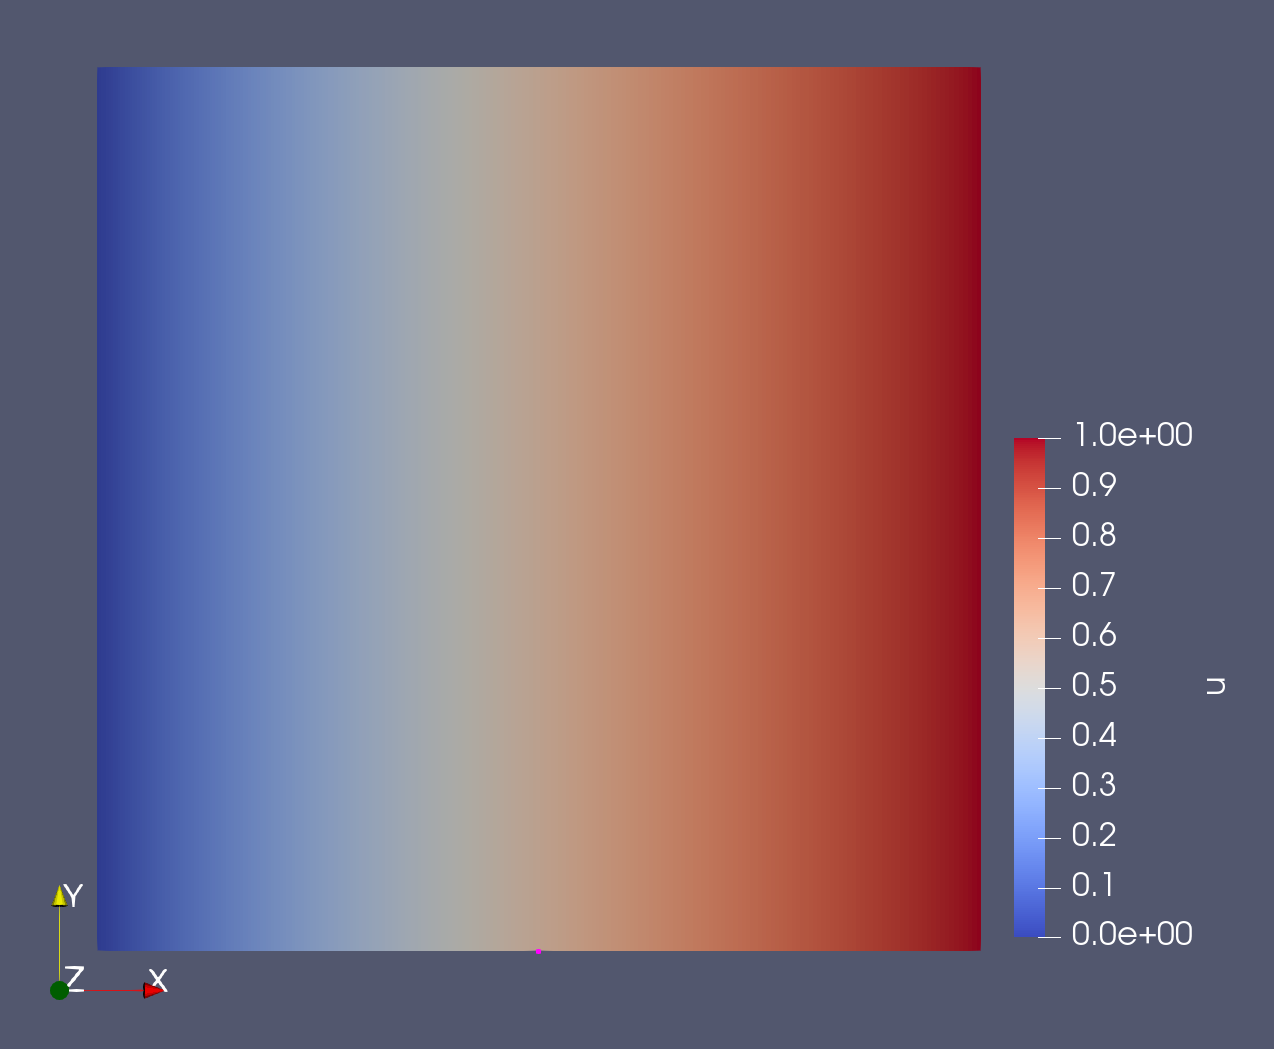
\includegraphics[width=0.6\textwidth]{Figures/result.png}
	\caption{Illustration of the solution of Nonlinear Poisson problem.}
	\label{fig_Rs}
\end{figure}
\begin{table}
	\caption{Numerical and exact solution for different $x$.}
	\label{tab1}
	\begin{center}
		\begin{tabular}{|c| c| c|} 
			\hline
			$x$ & $\mathbf{u}_{numerical}$ & $\mathbf{u}_{exact}$ \\ [0.7ex] 
			\hline\hline
			0 & 0.0 & 0.0 \\  [0.2ex] 
			\hline
			0.2 & 0.26491 & 0.264911064 \\ [0.2ex] 
			\hline
			0.4 & 0.48324 & 0.483239697 \\ [0.2ex] 
			\hline
			0.6 & 0.67332 & 0.673320053 \\ [0.2ex] 
			\hline
			0.8 & 0.84391 & 0.843908891 \\ [0.2ex] 
			\hline
			1.0 & 1.0 & 1.0 \\ [0.2ex] 
			\hline
		\end{tabular}
	\end{center}
\end{table}






\bibliographystyle{unsrt}
\bibliography{ref}
\end{document}
